\documentclass[a4paper,10pt]{report}
\usepackage[utf8]{inputenc}
\usepackage[english]{babel}
\usepackage[english]{isodate}
\usepackage{graphicx}
\usepackage{listings}
\usepackage[parfill]{parskip}
\usepackage{url}
%opening
\title{Relation Extraction using MultiR}
\author{}
\usepackage{xcolor}
\usepackage{color}
\newcommand{\hilight}[1]{\colorbox{yellow}{#1}}
\colorlet{punct}{red!60!black}
\definecolor{background}{HTML}{EEEEEE}
\definecolor{delim}{RGB}{20,105,176}
\definecolor{mygreen}{rgb}{0,0.6,0}
\definecolor{mygray}{rgb}{0.5,0.5,0.5}
\definecolor{mauve}{rgb}{0.58,0,0.82}
\definecolor{delim}{RGB}{20,105,176}
\definecolor{dkgreen}{rgb}{0,0.6,0}
\colorlet{numb}{magenta!60!black}

\lstdefinelanguage{json}{
    basicstyle=\normalfont\ttfamily,
    numbers=left,
    numberstyle=\scriptsize,
    stepnumber=1,
    numbersep=8pt,
    showstringspaces=false,
    breaklines=true,
    frame=lines,
    backgroundcolor=\color{background},
    literate=
     *{0}{{{\color{numb}0}}}{1}
      {1}{{{\color{numb}1}}}{1}
      {2}{{{\color{numb}2}}}{1}
      {3}{{{\color{numb}3}}}{1}
      {4}{{{\color{numb}4}}}{1}
      {5}{{{\color{numb}5}}}{1}
      {6}{{{\color{numb}6}}}{1}
      {7}{{{\color{numb}7}}}{1}
      {8}{{{\color{numb}8}}}{1}
      {9}{{{\color{numb}9}}}{1}
      {:}{{{\color{punct}{:}}}}{1}
      {,}{{{\color{punct}{,}}}}{1}
      {\{}{{{\color{delim}{\{}}}}{1}
      {\}}{{{\color{delim}{\}}}}}{1}
      {[}{{{\color{delim}{[}}}}{1}
      {]}{{{\color{delim}{]}}}}{1},
}
\lstset{frame=tb,
  language=Java,
  aboveskip=3mm,
  belowskip=3mm,
  showstringspaces=false,
  columns=flexible,
  basicstyle={\small\ttfamily},
  numbers=none,
  numberstyle=\tiny\color{gray},
  keywordstyle=\color{blue},
  commentstyle=\color{dkgreen},
  stringstyle=\color{mauve},
  breaklines=true,
  breakatwhitespace=true
  tabsize=3
}

\begin{document}
\maketitle

\begin{abstract}

\end{abstract}

\newpage
\chapter{Sg}
\section{Bird's eye view of things}

There are 2 separate repositories : MultirFramework and MultirExperiments. Latter is the latest version and the one you should be using for development. 

\subsection{Training}
\begin{itemize}
 \item Training
 
 The diagram below summarizes the process. The document is an attempt to explain the various black boxes. 
\begin{figure}[h]
 \centering
 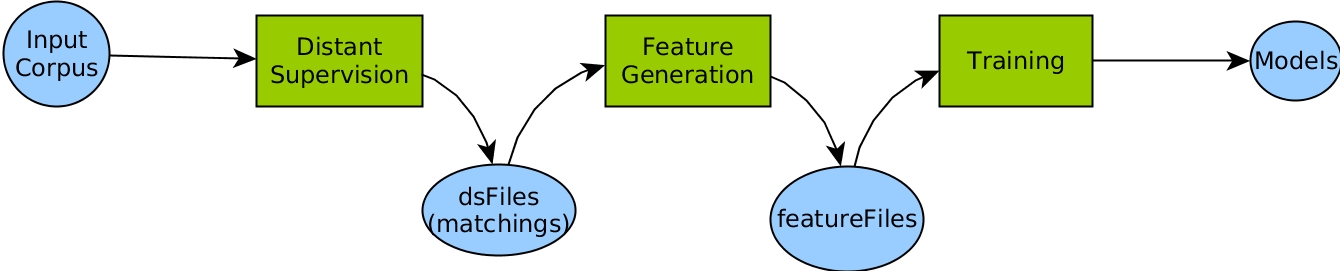
\includegraphics[bb=0 0 1109 107,scale=0.3,keepaspectratio=true]{./trainpipe.jpg}
 % trainpipe.jpg: 1109x107 pixel, 72dpi, 39.12x3.77 cm, bb=0 0 1109 107
 \caption{The Distant supervision training process}
 \label{fig:1}
\end{figure}
The file \url{https://github.com/knowitall/MultirExperiments/blob/master/src/main/java/edu/washington/multir/experiment/Experiment.java} is a good place to start.
It covers basically the whole of the Distant supervision pipeline. 

\subsection{Extraction}
TODO
 \end{itemize}
\section{Setting the stage}
There are several ways of implementing each of the blackboxes shown in the figure above. Thus, before starting, we need to decide on which implementations to use for each of them.
Once we have zeroed in on the choices, we need to supply this information to the orchestrator. The way we do that in the current setup is via a configuration file, which is essentially
a json file consisting of key value pairs. Keys are the black boxes and the values are the particular implementation to use. 

As the diagram shows, the Distant supervision process (ds process henceforth) also needs to know where is the corpus, the kb and what to call the intermediate files. 
All of this is also supplied by the configuration file. A standard configuration file will look as follows : 
\begin{lstlisting}[language=json,firstnumber=1]
{
  "corpusPath" :
"jdbc:derby:/mnt/a99/d0/aman/multir-exp-second/MultirExperiments-master/data/FullCorpus-First100Sentences",
  "train" : "true",
  "testDocumentsFile" :
"data/emptyFile",
  "fg" :
"edu.washington.multirframework.featuregeneration.DefaultFeatureGenerator",
  "ai" :
"edu.washington.multirframework.argumentidentification.NERArgumentIdentification",
  "rm" :
"edu.washington.multirframework.argumentidentification.NERRelationMatching",
  "nec" :
"edu.washington.multirframework.distantsupervision.NegativeExampleCollectionByRatio",
  "necRatio" : "0.25",
  "kbRelFile" : "data/kb/kb-facts-train.tsv.gz",
  "kbEntityFile" : "data/kb/entity-names-train.tsv.gz",
  "targetRelFile" : "data/kb/target-relations.tsv",
  "typeRelMap" : null,
  "sigs" : [
"edu.washington.multirframework.argumentidentification.DefaultSententialInstanceGeneration"
],
  "dsFiles" : [
"data/training-instances.tsv.gz"
],
  "featureFiles" : [
"data/training-instances-features.tsv"
],
  "models" : [
"data/multir-extractor" ],
  "cis" :
"edu.washington.multirframework.corpus.DefaultCorpusInformationSpecification",
  "si" : [
"edu.washington.multirframework.corpus.SentNamedEntityLinkingInformation",
"edu.washington.multirframework.corpus.SentFreebaseNotableTypeInformation"
],
  "ti" : [ "edu.washington.multirframework.corpus.TokenChunkInformation" ],
  "di" : [ ],
  "useFiger" : "false"
}
\end{lstlisting}
We will be referring to the configuration file as and when required.
\chapter{The Distant supervision process}
The first block of the pipeline, Distant supervision is responsible for reading the corpus and generating matching the sentence with the KB.
In this chapter, we look at how MultiR handles the whole process.
\section{Distant supervision process}
\subsection{Responsibilities} 
We start with a quick enumeration of steps involved in the process.
\begin{enumerate}
 \item Read the corpus
 \item Iterate over it sentence by sentence
 \item Find named entities pairs in each sentence
 \item Match the pairs found in step 4 to the facts that you know about entities (a.k.a the knowledge base)
 \item Dump matched relations for each sentence in a separate file \footnote{This file is specified in the configuration file by the property ``dsFiles``. The Distant supervision process runs only if this file does not exists.
} (to be used in training)
\end{enumerate}
We now read through the code and match the steps listed above with actual implementation.
\subsection{Code}
It will be easier to follow the code if you take the following at the moment as gospel's truth : 
\hilight{Annotation} is a document with attached information, \hilight{CoreMap} is a sentence with attached information, \hilight{CoreLabel} is a word with attached information. 
We plan to define these in detail in a separate chapter. We do not follow a strict dfs order while explaining the code; some method calls are skipped for brevity. 

\begin{lstlisting}[language=java]
DistantSupervision ds = new DistantSupervision(ai, sigs.get(0), rm, nec);
ds.run(DSFiles.get(0), kb, corpus)				
\end{lstlisting}
The above lines in experiment.java kickstart the whole process. Once inside the run method of DistantSupervision, things proceed as follows : 

\subsubsection{Iterating over documents}
First of all, we go to the corpus to get an iterator of the documents.

\begin{lstlisting}[language=java]
Iterator<Annotation> di = c.getDocumentIterator();
while(di.hasNext()) {
  Annotation d = di.next(); //get the next document
  List<CoreMap> sentences = d.get(CoreAnnotations.SentencesAnnotation.class); //get the sentences in the document
  List<NegativeAnnotation> documentNegativeExamples = new ArrayList<>(); //create space for negative annon in this doc
  List<Pair<Triple<KBArgument,KBArgument,String>,Integer>> documentPositiveExamples = new ArrayList<>(); 
\end{lstlisting}
Iterate over the corpus document by document. The document iterator is returned with the help of Corpus.java and CorpusHandler.java. These classes abstract the Apache derby database
from the user. 
\subsection{Identifying entities of interest in text}
\begin{lstlisting}[language=java]
for(CoreMap sentence : sentences) {
	int sentGlobalID = sentence.get(SentGlobalID.class);			
	//argument identification
	List<Argument> arguments =  ai.identifyArguments(d,sentence);
	//sentential instance generation
	List<Pair<Argument,Argument>> sententialInstances = sig.generateSententialInstances(arguments, sentence);
	//relation matching
\end{lstlisting}
There are two crucial functions being used here.
\begin{itemize}
 \item	\textbf{identifyArguments} : NER based argument identifier returns a list of named entity arguments by scanning the annotated CoreMap (sentences) for CoreLabels (Words),  the property CoreAnnotations.NamedEntityAnnotation of each of the labels and only returning those words that have NER tags among those listed in relevantNER.
  \item \textbf{SententialInstanceGeneration} : Takes a list of arguments and a sentence (CoreMap, annotated sentence in the sfu nlplib parlance) and returns a list of pairs that are non overlapping along with the sentences. Also makes sure that two arguments that are actually the same are not added as apair.
  This is done by making sure that they don't have the same id.
\end{itemize}


\subsection{Matching relations}
\begin{lstlisting}[language=java]
List<Triple<KBArgument,KBArgument,String>> distantSupervisionAnnotations = 
	rm.matchRelations(sententialInstances,kb,sentence,d);
\end{lstlisting}

Once we have identified the entities of interest in each of the sentences, the next step is to create the distantly supervised training data. 
This involves taking the entity pairs of interest (obtained by SententialInstanceGeneration) and using the kb to see if there are any matches. 
The NERRelationMatching has pretty simple implementation. For each pair of entities, it first maps the entities to freebase ids and then queries the knowledge
base for all possible relations that exist between the entity pair.



\subsection{Adding sentence ids and finding negative examples}
\begin{lstlisting}[language=java]


//adding sentence IDs
List<Pair<Triple<KBArgument,KBArgument,String>,Integer>> dsAnnotationWithSentIDs = new ArrayList<>();
for(Triple<KBArgument,KBArgument,String> trip : distantSupervisionAnnotations){
	Integer i = new Integer(sentGlobalID);
	Pair<Triple<KBArgument,KBArgument,String>,Integer> p = new Pair<>(trip,i);
	dsAnnotationWithSentIDs.add(p);
}
//negative example annotations
List<NegativeAnnotation> negativeExampleAnnotations =
  findNegativeExampleAnnotations(sententialInstances,distantSupervisionAnnotations,kb,sentGlobalID);
documentNegativeExamples.addAll(negativeExampleAnnotations);
documentPositiveExamples.addAll(dsAnnotationWithSentIDs);				
\end{lstlisting}
The negative examples are formed by the entity pairs that appear together but are not there in the knowledge base.

\subsection{Writing the matches to the disk}
\begin{lstlisting}[language=java]
writeDistantSupervisionAnnotations(documentPositiveExamples,dsWriter);
writeNegativeExampleAnnotations(nec.filter(documentNegativeExamples,
  documentPositiveExamples,kb,sentences),dsWriter);
\end{lstlisting}

The matches are stored on the disk in the a tab separated file (tsv) which is compressed to a gz file. The file can be specified using 
dsFiles property in the configuration. For example, if the sentence is \textbf{''Pravda is a popular newspaper of Moscow``}, the match would be saved
as 
\begin{verbatim}
 
/m/013v50	0	0	Pravda	/m/04swd	5	5	Moscow	102	newsPaperIn

\end{verbatim}

We will use this example to again go through the activities that take place in the  Distant supervision blackbox to reach this state: this sentence would have been fetched from the 
corpus, Pravda and Moscow would have been identified as Named entities (ORG and LOC respectively), relation matching would have found an entry with these 2 entities
in the KB and finally, it will be written down in the file specified by dsFiles.



\chapter{Feature Generation}

\subsection{Starting}
The process of feature generation starts from 
\begin{lstlisting}[language=java]
public void run(List<String> dsFileNames, List<String> featureFileNames, Corpus c, CorpusInformationSpecification cis)
\end{lstlisting}

The first argument contains the list of matchings. You will expect that being here means that dsFileNames have been populated. 
The second argument is the list of files where the corresponding features have to be written.
Next we have objects that help in getting corpus information.

Once in run, the major step is 

\begin{lstlisting}[language=java]
List<SententialArgumentPair> saps = getSaps(dsFileNames,featureFileNames);
\end{lstlisting}
This is familiar sentential argument pair from distance supervision. Argument pairs again are an abstraction that 
contains types, offsets, the sentence id and other similar information. 

\subsection{Storing entity pairs in each sentence}
We next populate the following data structure : 

\begin{lstlisting}[language=java]
Map<Integer,List<SententialArgumentPair>> sapMap = new HashMap<>();
\end{lstlisting}

This is a mapping which given a sentene number, returns all the arguments that are there in that sentence. 

We then start iterating over the corpus. Recall that this is the same corpus that was used during distance supervision. 
\begin{lstlisting}[language=java]
//iterate over corpus
    	Iterator<Annotation> di = c.getDocumentIterator();
    	int docCount =0;
    	start = System.currentTimeMillis();
    	while(di.hasNext()){
    		Annotation doc = di.next();
\end{lstlisting}

\begin{lstlisting}[language=java]

    		List<CoreMap> sentences = doc.get(CoreAnnotations.SentencesAnnotation.class);
    		for(CoreMap sentence: sentences){
    				
    			Integer currSentID = sentence.get(SentGlobalID.class);
    			if(sapMap.containsKey(currSentID)){
    				System.out.println(sentence);
    				List<SententialArgumentPair> sentenceSaps = sapMap.get(currSentID);
    				writeFeatures(sentenceSaps,doc,sentence,writerMap);
    			}
    		}
    		docCount++;
\end{lstlisting}
The above piece of code iterates over the corpus sentence by sentence.
For a given sentence, the map created in the above step is used to extract all the entity pairs that
exists in a particular sentence. 
if a sentence has some entity pairs, we extract all of them and then call writeFeatures, supplying the list
of entity pairs just extracted.
Lets now see how things look in writeFeatures()


\subsection{Writing features to files : writeFeatures()}

\begin{lstlisting}[language=java]
 for(SententialArgumentPair sap : currentSaps){
			BufferedWriter bw = writerMap.get(sap.partitionID);

			List<String> features = fg.generateFeatures(sap.arg1Offsets.first,sap.arg1Offsets.second
					,sap.arg2Offsets.first,sap.arg2Offsets.second,sap.arg1ID,sap.arg2ID,sentence,doc);
			bw.write(makeFeatureString(sap,features)+"\n");
		}
\end{lstlisting}
The features are based upon the entity pairs that exists in a sentence. Thus, MultiR iterates over the list of entity pairs and 
iterates over them one by one, calling generateFeatures() for each of these entities. 

\subsection{Generating Features}
We will be discussing the generateFeatures() function of the default feature generator here. The signature of the function looks as follows :

\begin{lstlisting}[language=java]
public List<String> generateFeatures(Integer arg1StartOffset,
			Integer arg1EndOffset, Integer arg2StartOffset,
			Integer arg2EndOffset, String arg1ID, String arg2ID, CoreMap sentence, Annotation document) {
\end{lstlisting}

The generate features function is supplied with information like offset and IDs of the entities that form the pair, the sentence and the document involved. 
Also supplied are the annotated sentence. 
Then we iterate over the sentence token by token, and it is checked whether the current token is one of the argument. 
Next up, we iterate over the dependency parse information and record it into an array. 

Finally, a call is made to the OriginalMultirFeatureGenerator()
\begin{lstlisting}[language=java]
 originalMultirFeatures(tokenStrings, posTags, depParents, depTypes, arg1Pos, arg2Pos, arg1ner, arg2ner);
\end{lstlisting}



\end{document}
